%% 
%% Copyright 2007-2020 Elsevier Ltd
%% 
%% This file is part of the 'Elsarticle Bundle'.
%% ---------------------------------------------
%% 
%% It may be distributed under the conditions of the LaTeX Project Public
%% License, either version 1.2 of this license or (at your option) any
%% later version.  The latest version of this license is in
%%    http://www.latex-project.org/lppl.txt
%% and version 1.2 or later is part of all distributions of LaTeX
%% version 1999/12/01 or later.
%% 
%% The list of all files belonging to the 'Elsarticle Bundle' is
%% given in the file `manifest.txt'.
%% 

%% Template article for Elsevier's document class `elsarticle'
%% with numbered style bibliographic references
%% SP 2008/03/01
%%
%% 
%%
%% $Id: elsarticle-template-num.tex 190 2020-11-23 11:12:32Z rishi $
%%
%%
%%\documentclass[preprint,12pt]{elsarticle}

%% Use the option review to obtain double line spacing
%% \documentclass[authoryear,preprint,review,12pt]{elsarticle}

%% Use the options 1p,twocolumn; 3p; 3p,twocolumn; 5p; or 5p,twocolumn
%% for a journal layout:
%%\documentclass[final,1p,times]{elsarticle}
%%\documentclass[final,1p,times,twocolumn]{elsarticle}
%% \documentclass[final,3p,times]{elsarticle}
\documentclass[final,3p,times,twocolumn]{elsarticle}
%% \documentclass[final,5p,times]{elsarticle}
%%\documentclass[final,5p,times,twocolumn]{elsarticle}

%% For including figures, graphicx.sty has been loaded in
%% elsarticle.cls. If you prefer to use the old commands
%% please give \usepackage{epsfig}
\usepackage{epsfig}

%% The amssymb package provides various useful mathematical symbols
\usepackage{amssymb}
%% The amsthm package provides extended theorem environments
%% \usepackage{amsthm}

%% The lineno packages adds line numbers. Start line numbering with
%% \begin{linenumbers}, end it with \end{linenumbers}. Or switch it on
%% for the whole article with \linenumbers.
%% \usepackage{lineno}

\journal{Journal of Magnetic Resonance}

\begin{document}

\begin{frontmatter}

%% Title, authors and addresses

%% use the tnoteref command within \title for footnotes;
%% use the tnotetext command for theassociated footnote;
%% use the fnref command within \author or \address for footnotes;
%% use the fntext command for theassociated footnote;
%% use the corref command within \author for corresponding author footnotes;
%% use the cortext command for theassociated footnote;
%% use the ead command for the email address,
%% and the form \ead[url] for the home page:
%% \title{Title\tnoteref{label1}}
%% \tnotetext[label1]{}
%% \author{Name\corref{cor1}\fnref{label2}}
%% \ead{email address}
%% \ead[url]{home page}
%% \fntext[label2]{}
%% \cortext[cor1]{}
%% \affiliation{organization={},
%%             addressline={},
%%             city={},
%%             postcode={},
%%             state={},
%%             country={}}
%% \fntext[label3]{}

\title{Exploring SABRE-Enhanced Imaging with a Portable Clinical Low-Field MRI Scanner}

%% use optional labels to link authors explicitly to addresses:
%% \author[label1,label2]{}
%% \affiliation[label1]{organization={},https://www.overleaf.com/project/62f1747044f8baf53ab6bd58
%%             addressline={},
%%             city={},
%%             postcode={},
%%             state={},
%%             country={}}
%%
%% \affiliation[label2]{organization={},
%%             addressline={},
%%             city={},
%%             postcode={},
%%             state={},
%%             country={}}

\author[inst1]{Nadiya Iqbal}

\affiliation[inst1]{organization={Department of Chemistry and Biochemistry},%Department and Organization
            addressline={Southern Illinois University}, 
            city={Carbondale},
            postcode={62901}, 
            state={Illinois},
            country={USA}}

\author[inst1]{Drew Brittin}
\author[inst1]{Praveen Jayasuriya Daluwathumullagamage}
\author[inst1]{Anthony Petrilla}
\author[inst1]{Margret Pugh}
\author[inst1]{Shahabuddin Alam}
\author[inst1]{Ishani Senananyake}
\author[inst1]{Tobi Abdulgafar}
\author[inst1]{Zahid Siraj}

\affiliation[inst2]{organization={Hyperfine.io}}

\author[inst2]{Megan Poorman}
\author[inst2]{Laura Sacolick}

\affiliation[inst3]{organization={A.A. Martinos Center for Biomedical Imaging},
            addressline={Massachusetts General Hospital and Harvard Medical School}, 
            city={Boston},
            postcode={02129}, 
            state={MA},
            country={USA}}
\author[inst3]{Matthew S. Rosen}

\affiliation[inst4]{organization={Wayne State University and Karmanos Cancer Institute},%Department and Organization
            addressline={(KCI)}, 
            city={Detroit},
            state={MI},
            country={USA}}
\author[inst4]{Eduard Y. Chekmenev}
\author[inst1]{Boyd M. Goodson}

\begin{abstract}
Our present work explores SABRE-enhanced imaging using a point-of-care low-field magnetic resonance imaging scanner. We introduce a new method to quantify signal enhancement using known concentrations of water samples as calibration standards. Low-field MRI has gained renowned interest due to low magnetic field strength obviating the requirement for bulky, immobile and expensive hardware. However, signal strength, detection sensitivity and contrast limitations present ongoing challenges. One approach to mitigate the sensitivity and contrast limitations of conventional NMR/MRI is hyperpolarization, which involves the preparation of nuclear spin polarization levels that are above their equilibrium values. 
In this study, we investigate signal amplification by reversible exchange (SABRE) to quantify signal from images to calculate enhancement. 
\end{abstract}

%%Graphical abstract
\begin{graphicalabstract}
\includegraphics{grabs}
\end{graphicalabstract}

%%Research highlights
\begin{highlights}
\item Research highlight 1
\item Research highlight 2
\end{highlights}

\begin{keyword}
%% keywords here, in the form: keyword \sep keyword
Low-field Magnetic Resonance Imaging \sep Signal Amplification by Reversible Exchange \sep Nuclear Magentic Resonance 
%% PACS codes here, in the form: \PACS code \sep code
\PACS 0000 \sep 1111
%% MSC codes here, in the form: \MSC code \sep code
%% or \MSC[2008] code \sep code (2000 is the default)
\MSC 0000 \sep 1111
\end{keyword}

\end{frontmatter}

%% \linenumbers

%% main text


\section{Introduction}
Magnetic Resonance Imaging (MRI) is a non-invasive imaging technique that provides exquisite high-resolution images of anatomical features, function, and pathology of soft tissues in the body without the use of ionizing radiation. The increasingly stronger magnets used in most clinical scanners ($\sim$1–7 T) are expensive, bulky, and immobile, and scans can be time-consuming and confining for many patients.  These  magnetic fields: along with concomitantly higher RF resonance frequencies, can present safety concerns in some circumstances, as well as contraindications for a number of patients and health conditions. 
\par Low field (LF) MRI\cite{blanchard2021lower}\cite{coffey2013low}\cite{coffey2014high}\cite{barskiy2014situ}\cite{lehmkuhl2020sabre} has gained renewed interest because it can potentially obviate all these limitations; however, signal strength, detection sensitivity and contrast limitations present ongoing challenges to many low-field MRI technologies and their applications. One approach to mitigate sensitivity and contrast limitations of the conventional nuclear magnetic resonance (NMR) or MRI is hyperpolarization, which involves the preparation of nuclear spin polarization levels that are far above their equilibrium levels resulting in a large gain in signal \cite{lehmkuhl2020sabre}\cite{nikolaou2015nmr} by orders of magnitude. Moreover, because the magnetization is endowed by a given hyperpolarization method and not the magnet, hyperpolarized (HP) low-field MRI has proven it can sometimes be more sensitive than high-field MRI\cite{coffey2013low} and thus, hyperpolarization can be highly synergistic with low-field MRI, if the hyperpolarization technique is itself low-cost, rapid, and portable\cite{barskiy2014situ}\cite{lehmkuhl2020sabre}\cite{nikolaou2015nmr}. 
\par One such approach is signal amplification by reversible exchange (SABRE)\cite{adams2009reversible}. In SABRE, parahydrogen (pH$_{\mathrm{2}}$) and molecular substrates are transiently bound to organometallic complexes (ususally an Ir-based catalyst) allowing spin order to transfer spontaneously from pH$_{\mathrm{2}}$ to substrates when placed within an appropriate magnetic field. Hyperpolarization can enable both faster acquisition and higher signal with low concentrations of substrate. We have sited a portable, point-of-care 64 mT clinical MRI scanner (Hyperfine) in the Goodson Lab at SIUC. This type of scanner has already been demonstrated in clinical settings for bed-side imaging, including of brain injury and cerebral hemorrhage \cite{sheth2020first}\cite{mazurek2021portable}. Here we are investigating the potential for adapting this type of MRI scanner for use with hyperpolarized substances in biomedical studies. 
\par The present study investigates 1H SABRE hyperpolarized pyrazine and nicotinamide integrated with the scanner and a pH$_{\mathrm{2}}$-bubbling SABRE setup\cite{truong2014irreversible} wherein the substrate samples were placed inside a shortened 5 mm NMR tube (pH$_{\mathrm{2}}$ produced by an ~86\% pH$_{\mathrm{2}}$ generator\cite{birchall2020high}), allowing the tube to be placed vertically within the scanner’s head coil. Pyrazine is a well-known test substrate for SABRE and nicotinamide (Vitamin B3-amide) can be a potential imaging agent which is an intrinsically safe clinical agent that has already been used in pharmacological doses with a low incidence of side effects and toxicity over many years\cite{cosmetic2005final}.

\begin{figure}
    \centering
    \includegraphics[width=\linewidth]{mri.png}
    \caption{The portable point-of-care 64mT clinical MRI scanner (Hyperfine "Lucy") in the Goodson Lab at SIUC. }
    \label{fig:my_label}
\end{figure}

\begin{figure}
    \centering
    \includegraphics[width=\linewidth]{Picture3.png}
    \caption{A simplified cartoon showing signal amplification by reversible exchange using the Ir catalyst transferring polarization transiently to pyrazine (py) and nicotinamide (nico). }
    \label{fig:my_label}
\end{figure}

Following 1H SABRE detection using a benchtop spectrometer, the sample was transferred to the MRI scanner where it was imaged in situ\cite{coffey2014high}\cite{barskiy2014situ}\cite{kovtunov2017imaging} at 64 mT under conditions of low flow (20 sccm) pH$_{\mathrm{2}}$ continuous bubbling and images with a resolution of 1.5x1.5x5mm\textsuperscript{3} was obtained when a fast spin echo (FSE) sequence was used to image for 5min. Low-field scanners suffer much less from susceptibility distortions, enabling imaging with gentle bubbling.
The acquired images were then processed using openCV to measure enhancements by hyperpolarization for pyrazine and nicotinamide.
A few-hundred fold enhancement is evident from the fact that the signal-per-pixel in the tube (near-zero without pH$_{\mathrm{2}}$) is similar to that obtained with pure water. 
\par The ideal magnetic field strength for SABRE j-scalar coupling network to transfer polarization is roughly between $\sim$6-8mT. The next set of experiments involved bubbling pH$_{\mathrm{2}}$ just outside the headcoil (measured at 65G) for 30 seconds and imaged using the scanner (64mT) using a spin density map. The acquisition time for the experiment was 15s with a resolution of 1x1x3.5 mm\textsuperscript{3}. 

\section{Methods}

\subsection{Quantity Signal Generation}

All experiments were conducted by bubbling para-hydrogen gas through a solution of 100 mM substrate, pyrazine (py) and nicotinamide (nico) , in CD$_{\mathrm{3}}$OD with 5.7 mM
Ir(IMes)(COD)Cl as catalyst for SABRE in a shortened 5 mm NMR tube placed vertically within the scanner’s head coil. 
\begin{figure}
    \centering
    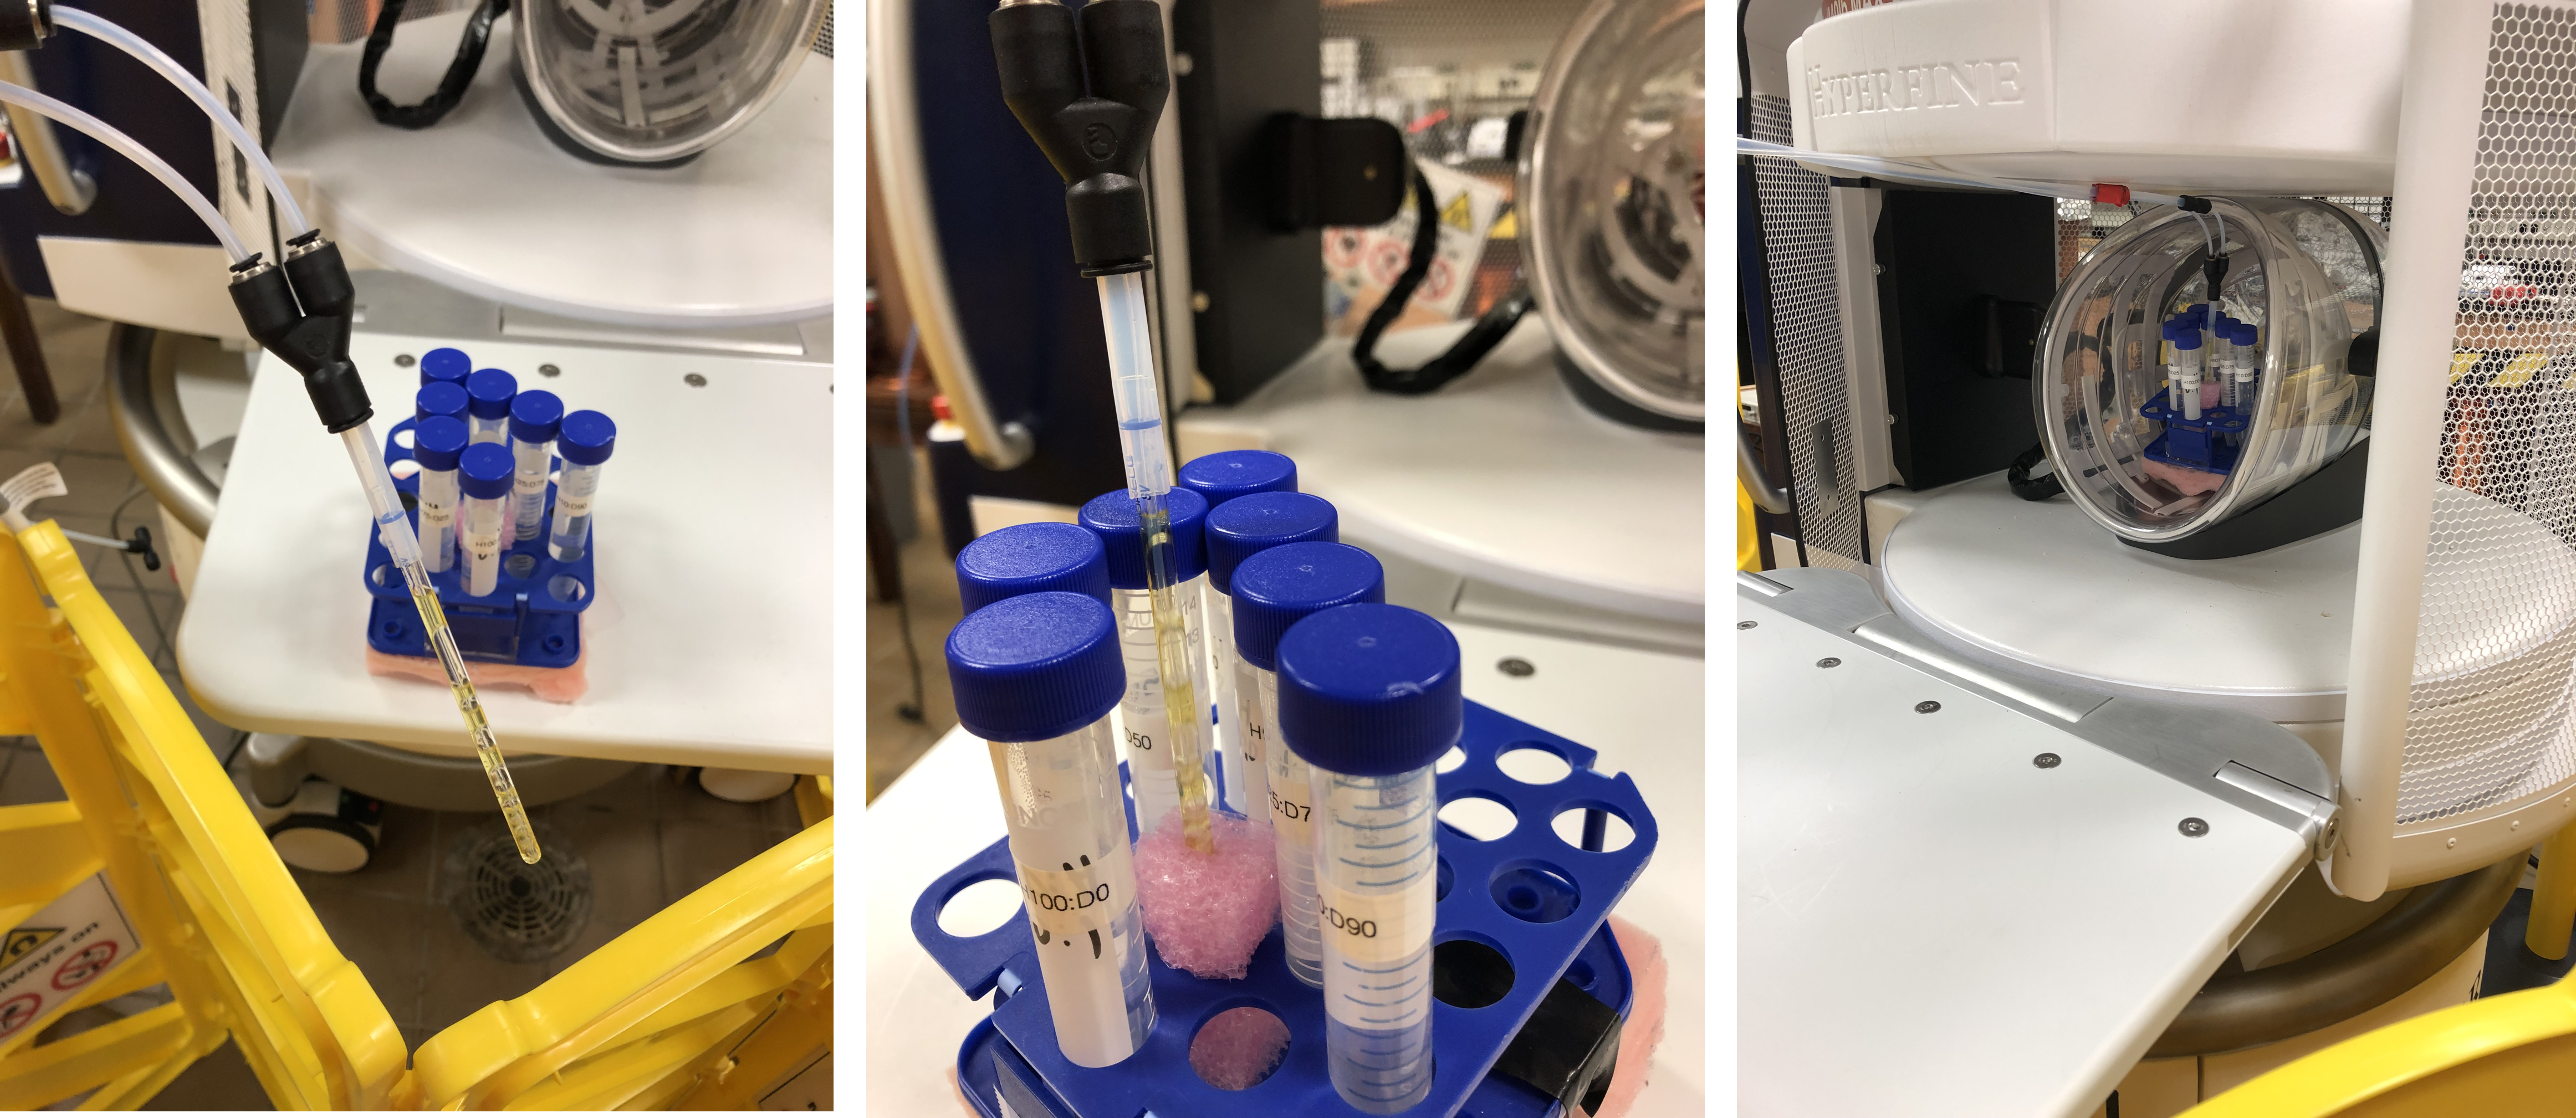
\includegraphics[width=\linewidth]{sabreinhyperfine.png}
    \caption{Continous pH$_{\mathrm{2}}$) bubbling and SABRE setup of the pyrazine sample placed inside a shortened 5mm NMR tube.}
    \label{fig:my_label}
\end{figure}

The SABRE catalyst was activated for 20 min by continuously bubbling pH$_{\mathrm{2}}$ into the sample at 90sccm. Once activated, a multichannel nanalysis benchtop 60 MHz NMR spectrometer was used to perform a single scan SABRE-enhanced 1H NMR spectroscopy experiment. The parameters for SABRE were optimized for pyrazine and nicotinamide and following its confirmation, samples were transferred to the 64mT Hyperfine MRI scanner. 
A fast spin echo (FSE) which took 5 min at 20sccm in continuous bubbling and a spin density map were used to obtain SABRE-enhanced images with different parameters. To quantify signal, falcon tube samples containing fractions of H$_{\mathrm{2}}$O/D$_{\mathrm{2}}$O (100\%, 90\%, 75\%, 50\%, 25\%, 10\% and 0\%) were used along with the SABRE tube.

\subsection{Image Processing}

The Hpyerfine  MRI scanner processes the raw quantity signals to \texttt{.dcm} (DICOM) images using a proprietary data reduction pipeline which was not exposed to the researchers. These files can be viewed and exported to a local drive via a proprietary web application. This web application does not posses the capabilities to further process the DICOM images. For the purpose of this work, these images were exported from the web application to a local drive and processed by a image processing pipeline developed by the researchers. 

The Python language version of \texttt{.OpenCV} was used for this image processing pipeline \cite{opencv_library}. \texttt{.Pydicom} \cite{mason2011t} was used for DICOM image conversion to Python arrays. Additionally, libraries such as \texttt{.matplotlib} was used for plotting intermediate and final results. 

The exported DICOM file from the web application contained multiple coronal views of the tubes with varying levels of image intensity. The view with the maximum total image intensity was selected from this list of views. The portion of the image containing the tubes was isolated to a 70x50 pixel region. The region of the image outside this isolated pixel region did not contain useful information regarding the tubes and was thus discarded.

ADD RAW IMAGE HERE

The raw image data which comprised 0 to 40,000 grayscale values was normalised to 256 levels. Image threshholding was used to develop a binary mask of the test tubes. This mask was then used to isolate the contours of each test tube in the chosen coronal view. These contours were approximately circular. Deviations from the circular shape were due to local variations in concentration across the coronal view of test tube resulting in image artefacts (noise). 

ADD NORMALISED IMAGE HERE

Not all test tubes were isolated using a single binary mask. The broad range of gray values resulted in a significantly different threshold for masking the tubes with the highest intensities compared to a single tube with the lowest image intensity. Thus a second mask was used to isolate the tube with the lowest image intensity.

ADD BINARY MASK HERE 

The coronal view of the tubes were used to plot colour maps using matplotlib. The plotted maps were then used to normalize to a 256 pixel array. The normalized data was averaged by isolating pixel under each isolated area and pixel values between a minimum and maximum value was used to threshold. Then the obtained average signal was plotted against the concentration of 1H to obtain a calibration curve. 
The calibration curve was then used to quantify polarization enhancement. 

\section{Results}
A linear dependence was found for the amount of signal obtained measured from a given H$_{\mathrm{2}}$O/D$_{\mathrm{2}}$O phantom and the $^{\mathrm{1}}$H concentration. This relationship can be used to quantify the product if concentration and polarization from a given region of an image with a given region of an image with good reliability: $y=( [H]*P )x+b$; a P (relative) value of $^{\mathrm{1}}$H was used for thermally polarized spins. Following confirmation of $^{\mathrm{1}}$H SABRE on the benchtop spectrometer, SABRE-MRI was demonstrated with pyrazine following sample transfer to the 64mT MRI and in-situ imaging under continous but reduced pH$_{\mathrm{2}}$ flow (20 sccm), yielding an enhancement of $\sim$240-fold; as low-field scanners suffer much less susceptibility distortions, enabling imaging with gentle bubbling. 
\par Smaller SABRE enhancements were observed for nicotinamide at lower concentrations ($\sim$110-fold) in the MRI. Reduced MRI signal may also reflect the fact that when pH$_{\mathrm{2}}$ bubbling is performed at the imaging field (64mT), there are both positive and negative SABRE enhancements in corresponding to the the benchtop NMR spectra, which may partially cancel out in the MRI scanner. 
SABRE performed at $\sim$6.5mT showed higher enhancement (nanalysis) in comparison to in-situ imaging. Faster image acquisition has allowed to acquire images of sabre enhanced pyrazine and nicotinamide after 30s of bubbling pH$_{\mathrm{2}}$ with a 1.0x1.0x3.5mm\textsuperscript{3} image resolution in 15s.
\section{Conclusions}
The use of phantoms containing known and varying quantities of H versus D spins enabled development of a simple approach to quantify the product of concentration and polarization from a given region of an image with good reliability. Pyrazine and nicotinamide were successfully hyperpolarized using SABRE under continous pH$_{\mathrm{2}}$ bubbling conditions and the HP agents were imaged using a low-field (64mT) clinical MRI scanner. 
The absence of signal in a control image using deutarated pyrazine supports the conclusion that the pH$_{\mathrm{2}}$ enhanced MRI signal is coming from SABRE hyperpolarized pyrazine and not from hyperpolarized oH$_{\mathrm{2}}$ or hydrides, or HP signals from oH$_{\mathrm{2}}$.

%\label{sec:sample1}
 

%Lorem ipsum dolor sit amet, consectetur adipiscing elit, sed do eiusmod tempor incididunt ut labore et dolore magna aliqua. Ut enim ad minim veniam, quis nostrud exercitation ullamco laboris nisi ut aliquip ex ea commodo consequat. Duis aute irure dolor in reprehenderit in voluptate velit esse cillum dolore eu fugiat nulla pariatur. Excepteur sint occaecat cupidatat non proident, sunt in culpa qui officia deserunt mollit anim id est laborum see appendix~\ref{sec:sample:appendix}.

%% The Appendices part is started with the command \appendix;
%% appendix sections are then done as normal sections
\appendix

\section{Sample Appendix Section}
\label{sec:sample:appendix}
Lorem ipsum dolor sit amet, consectetur adipiscing elit, sed do eiusmod tempor section incididunt ut labore et dolore magna aliqua. Ut enim ad minim veniam, quis nostrud exercitation ullamco laboris nisi ut aliquip ex ea commodo consequat. Duis aute irure dolor in reprehenderit in voluptate velit esse cillum dolore eu fugiat nulla pariatur. Excepteur sint occaecat cupidatat non proident, sunt in culpa qui officia deserunt mollit anim id est laborum.

%% If you have bibdatabase file and want bibtex to generate the
%% bibitems, please use
%%
 \bibliographystyle{elsarticle-num} 
 \bibliography{cas-refs}

%% else use the following coding to input the bibitems directly in the
%% TeX file.

% \begin{thebibliography}{00}

% %% \bibitem{label}
% %% Text of bibliographic item

% \bibitem{}

% \end{thebibliography}
\end{document}
\endinput
%%
%% End of file `elsarticle-template-num.tex'.
